% LLM-YARA Pipeline Diagram
% Compile: pdflatex pipeline.tex
\documentclass[border=5pt]{standalone}
\usepackage{tikz}
\usepackage{pgfplots}
\pgfplotsset{compat=1.18}
\usetikzlibrary{arrows.meta, positioning, shapes.geometric, backgrounds, fit, calc}

% ── Colour palette ──────────────────────────────────────────────────
\definecolor{datablue}{HTML}{3B82F6}
\definecolor{databluefill}{HTML}{DBEAFE}
\definecolor{llmorange}{HTML}{EA580C}
\definecolor{llmorangefill}{HTML}{FFEDD5}
\definecolor{evalgreen}{HTML}{16A34A}
\definecolor{evalgreenfill}{HTML}{DCFCE7}
\definecolor{gateamber}{HTML}{D97706}
\definecolor{gatefill}{HTML}{FEF3C7}
\definecolor{rejectred}{HTML}{DC2626}
\definecolor{acceptgreen}{HTML}{16A34A}
\definecolor{arrowgray}{HTML}{6B7280}
\definecolor{substepgray}{HTML}{F3F4F6}
\definecolor{looppurple}{HTML}{7C3AED}

\begin{document}
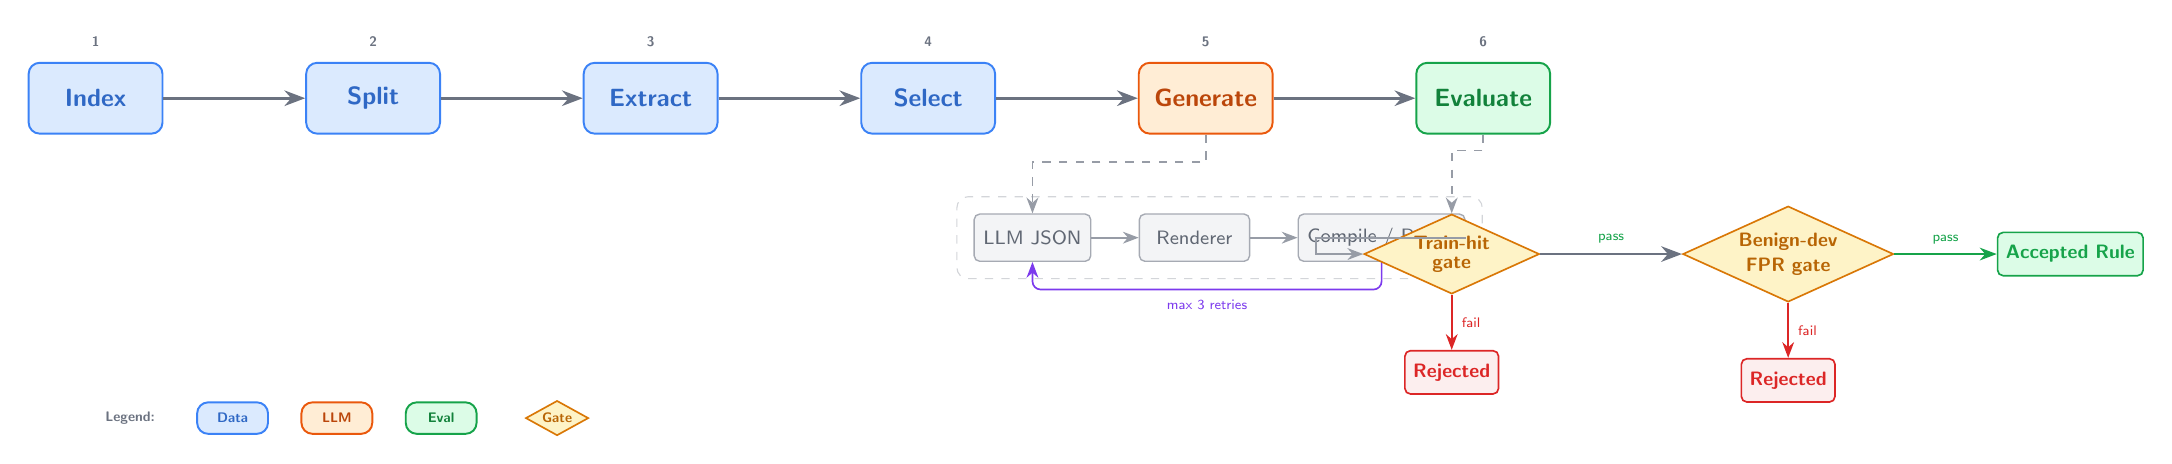
\begin{tikzpicture}[
    >=Stealth,
    node distance=1.6cm and 1.8cm,
    font=\sffamily\small,
    % ── stage styles ──
    datastage/.style={
        draw=datablue, fill=databluefill, text=datablue!80!black,
        rounded corners=4pt, minimum height=0.9cm, minimum width=1.7cm,
        line width=0.7pt, font=\sffamily\small\bfseries,
    },
    llmstage/.style={
        draw=llmorange, fill=llmorangefill, text=llmorange!80!black,
        rounded corners=4pt, minimum height=0.9cm, minimum width=1.7cm,
        line width=0.7pt, font=\sffamily\small\bfseries,
    },
    evalstage/.style={
        draw=evalgreen, fill=evalgreenfill, text=evalgreen!80!black,
        rounded corners=4pt, minimum height=0.9cm, minimum width=1.7cm,
        line width=0.7pt, font=\sffamily\small\bfseries,
    },
    % ── arrows ──
    stage arrow/.style={
        ->, arrowgray, line width=1pt,
    },
    % ── substep style ──
    substep/.style={
        draw=arrowgray!60, fill=substepgray, text=arrowgray!90!black,
        rounded corners=2pt, minimum height=0.6cm, minimum width=1.4cm,
        line width=0.5pt, font=\sffamily\scriptsize,
    },
    % ── gate style ──
    gate/.style={
        draw=gateamber, fill=gatefill, text=gateamber!85!black,
        diamond, aspect=2.2, minimum width=1.2cm, minimum height=0.7cm,
        line width=0.6pt, font=\sffamily\scriptsize\bfseries,
        inner sep=1pt,
    },
    % ── outcome ──
    outcome/.style={
        rounded corners=2pt, minimum height=0.55cm, minimum width=1.1cm,
        line width=0.6pt, font=\sffamily\scriptsize\bfseries, inner sep=3pt,
    },
]

% ══════════════════════════════════════════════════════════════════════
%  Top row — main pipeline stages
% ══════════════════════════════════════════════════════════════════════
\node[datastage]                (index)    {Index};
\node[datastage, right=of index]   (split)    {Split};
\node[datastage, right=of split]   (extract)  {Extract};
\node[datastage, right=of extract] (select)   {Select};
\node[llmstage, right=of select]   (generate) {Generate};
\node[evalstage, right=of generate](evaluate) {Evaluate};

% ── arrows between stages ──
\foreach \a/\b in {index/split, split/extract, extract/select, select/generate, generate/evaluate}{
    \draw[stage arrow] (\a) -- (\b);
}

% ── stage numbers ──
\foreach \n/\stage in {1/index, 2/split, 3/extract, 4/select, 5/generate, 6/evaluate}{
    \node[above=2pt of \stage, font=\sffamily\tiny\bfseries, text=arrowgray]
        {\n};
}

% ══════════════════════════════════════════════════════════════════════
%  Sub-steps below "Generate"
% ══════════════════════════════════════════════════════════════════════
\node[substep, below=1.0cm of generate, xshift=-2.2cm] (llmjson)  {LLM JSON};
\node[substep, right=0.6cm of llmjson]                 (renderer) {Renderer};
\node[substep, right=0.6cm of renderer]                (compile)  {Compile / Repair};

% ── arrows among substeps ──
\draw[->, arrowgray!70, line width=0.6pt] (llmjson)  -- (renderer);
\draw[->, arrowgray!70, line width=0.6pt] (renderer) -- (compile);

% ── connection from Generate stage down ──
\draw[->, arrowgray!70, line width=0.6pt, dashed]
    (generate.south) -- ++(0,-0.35) -| (llmjson.north);

% ── repair loop (max 3) ──
\draw[->, looppurple, line width=0.6pt, rounded corners=3pt]
    (compile.south) -- ++(0,-0.35) -| node[pos=0.25, below, font=\sffamily\tiny,
    text=looppurple]{max 3 retries} (llmjson.south);

% ══════════════════════════════════════════════════════════════════════
%  Gates below "Evaluate"
% ══════════════════════════════════════════════════════════════════════
\node[gate, below=1.0cm of evaluate, xshift=-0.4cm] (traingate) {%
    \shortstack{Train-hit\\gate}};
\node[gate, right=1.8cm of traingate] (fprgate) {%
    \shortstack{Benign-dev\\FPR gate}};

% ── connection from Evaluate down ──
\draw[->, arrowgray!70, line width=0.6pt, dashed]
    (evaluate.south) -- ++(0,-0.2) -| (traingate.north);

% ── arrow between gates ──
\draw[stage arrow] (traingate) -- node[above, font=\sffamily\tiny, text=acceptgreen]{pass} (fprgate);

% ── Accepted output ──
\node[outcome, draw=acceptgreen, fill=evalgreenfill, text=acceptgreen,
      right=1.3cm of fprgate] (accepted) {Accepted Rule};
\draw[->, acceptgreen, line width=0.7pt]
    (fprgate) -- node[above, font=\sffamily\tiny, text=acceptgreen]{pass} (accepted);

% ── Rejected outputs ──
\node[outcome, draw=rejectred, fill=rejectred!8, text=rejectred,
      below=0.7cm of traingate] (rej1) {Rejected};
\draw[->, rejectred, line width=0.6pt]
    (traingate.south) -- node[right, font=\sffamily\tiny, text=rejectred]{fail} (rej1);

\node[outcome, draw=rejectred, fill=rejectred!8, text=rejectred,
      below=0.7cm of fprgate] (rej2) {Rejected};
\draw[->, rejectred, line width=0.6pt]
    (fprgate.south) -- node[right, font=\sffamily\tiny, text=rejectred]{fail} (rej2);

% ── compile output feeds into gates ──
\draw[->, arrowgray!70, line width=0.6pt]
    (compile.east) -| ([xshift=-0.6cm]traingate.west) -- (traingate.west);

% ══════════════════════════════════════════════════════════════════════
%  Background boxes for legend clarity
% ══════════════════════════════════════════════════════════════════════
\begin{scope}[on background layer]
    % substep region
    \node[fit=(llmjson)(compile), inner sep=6pt, rounded corners=4pt,
          draw=arrowgray!30, fill=white, dashed, line width=0.4pt] {};
\end{scope}

% ══════════════════════════════════════════════════════════════════════
%  Legend
% ══════════════════════════════════════════════════════════════════════
\node[below=3.6cm of index, anchor=west, font=\sffamily\tiny\bfseries, text=arrowgray]
    (legendtitle) {Legend:};
\node[datastage, right=0.4cm of legendtitle, minimum height=0.4cm, minimum width=0.9cm,
      font=\sffamily\tiny\bfseries] (l1) {Data};
\node[llmstage, right=0.4cm of l1, minimum height=0.4cm, minimum width=0.9cm,
      font=\sffamily\tiny\bfseries] (l2) {LLM};
\node[evalstage, right=0.4cm of l2, minimum height=0.4cm, minimum width=0.9cm,
      font=\sffamily\tiny\bfseries] (l3) {Eval};
\node[gate, right=0.6cm of l3, minimum width=0.6cm, minimum height=0.3cm,
      font=\sffamily\tiny\bfseries, aspect=1.8] (l4) {Gate};

\end{tikzpicture}
\end{document}
